% !TEX root = ../root.tex

\chapter{Advanced: Splines on Lie Groups}

This is largely based on \cite{patron-perez_spline-based_2015, sommer_efficient_2020}.


\begin{figure}[h]
  \begin{center}
    \begin{tikzpicture}
      \foreach \n in {0,1,2,...,10}
        {
          \coordinate (T\n) at ($(0,0)+(\n*1cm,0)$) {};
          \draw ($(T\n)+(0,5pt)$) -- ($(T\n)-(0,5pt)$);
          \node at ($(T\n)-(0,3ex)$) {$t_{\n}$};
          \coordinate (P\n) at ($(0,2)+(\n*1cm,{sin(\n r)})$) {};
          \node at (P\n)[circle, fill, inner sep=1.5pt] {};
          \node at ([yshift=-5mm]P\n) {$\x_{\n}$};
        }
      \draw[-latex] (T0) -- (T10) -- ($(T10)+1.5*(1,0)$);
    \end{tikzpicture}
  \end{center}
\end{figure}

A B-spline interpolation of order $k$ is a function $\x(t) = \sum_{i=0}^N B_{i, k}(t) \x_{v(i)}$ where $\x_{v(i)} \in \mathbb{R}^n$ are \textbf{control points} for \textbf{knots} $t_i$, and $B_{i, k}(t)$ are \textbf{basis functions} recursively defined as

\begin{equation}
  \label{eq:b_spline_rec}
  \begin{aligned}
    B_{i, 0}(t) & = \begin{cases}
      1 & t_i \leq t < t_{i+1}, \\
      0 & \text{otherwise}.
    \end{cases}                                                                                \\
    B_{i, k}(t) & = \frac{t - t_i}{t_{i+k} - t_i} B_{i, k-1}(t) + \frac{t_{i+k+1} - t}{t_{i+k+1} - t_{i+1}} B_{i+1, k-1}(t).
  \end{aligned}
\end{equation}

The following are some well-known properties of B-splines:
\begin{itemize}
  \item $B_{i, k}(t)$ has finite support and is zero outside the interval $[t_{i}, t_{i+k+1})$,
  \item Inside this interval it is a piecewise polynomial of degree $k$,
  \item It is centered in the middle of that interval, it therefore makes sense to select $k$ odd and $v(i) = i + (k + 1) / 2$ so that $x_{v(i)}$ coincides with the maximum of $B_{i, k}(t)$ (c.f. Figure \ref{fig:bspline_nonzero}),
  \item $\sum_i B_{i, k}(t) = 1$ for all $t$,
\end{itemize}

We are interested in an expression for the coefficients of the polynomial $B_{i, k}(t)$. We pose that for \textbf{a fixed interval} $t \in [t_{i^*}, t_{i^*+1})$ we have scalar cofficients $\alpha^i_{i,k}$ such that
\begin{equation}
  \label{eq:basis_expression}
  B_{i, k}(t) = \sum_{l=0}^k \alpha^{l}_{i, k} \; u^l(t), \quad u(t) = \frac{t - t_{i^*}}{t_{i^*+1} - t_{i^*}}
\end{equation}
where $i \in \{ i^* - k, i^* - k + 1, \ldots, i^* \}$ are the indices for which $B_{i, k}(t)$ is non-zero on $[t_{i^*}, t_{i^*+1})$ (c.f. Figure \ref{fig:bspline_nonzero}). If we also introduce
\begin{equation}
  \label{eq:coeff_matrix_forms}
  \begin{aligned}
    N_{i, k}   & \coloneq \begin{bmatrix} \alpha_{i,k}^0 & \alpha_{i, k}^1 & \cdots & \alpha_{i, k}^k \end{bmatrix}^T \in \mathbb{R}^{k+1}    \\
    M_{i^*, k} & \coloneq \begin{bmatrix}
      N_{i^*-k, k} & N_{i^*-k+1, k} & \cdots & N_{i^*, k}
    \end{bmatrix} \in \mathbb{R}^{k+1, k+1}
  \end{aligned}
\end{equation}
we can write the value of a spline $x(t)$ for $t \in [t_{i^*}, t_{i^*+1}]$ as
\begin{equation}
  \begin{aligned}
    \x(t) = \sum_{j = 0}^n B_{j,k}(t) \x_{v(j)} = \sum_{j = i^*-k}^{i^*} B_{j,k}(t) \x_{v(j)} = \sum_{j = i^*-k}^{i^*} \sum_{l=0}^k \alpha_{j, k}^l u^l \x_{v(j)} =  \begin{bmatrix} 1 & u & \cdots & u^k \end{bmatrix} M_{i^*, k} \begin{bmatrix} \x_{v(i^* - k)} \\ \vdots \\ \x_{v(i^*)} \end{bmatrix}.
  \end{aligned}
\end{equation}

\begin{figure}[h]
  \begin{center}
    \footnotesize
    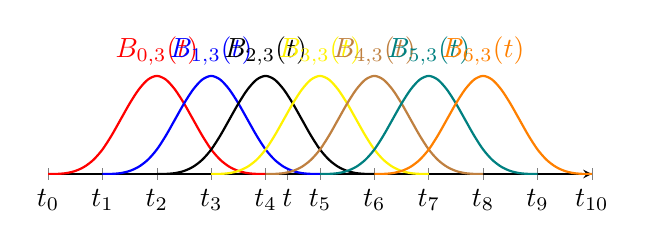
\begin{tikzpicture}[
        declare function={
            bspline3(\x) = and(0<=\x, \x<1) * (\x^3/6) +
            and(1<=\x, \x<2) * ((-3*(\x-1)^3+3*(\x-1)^2+3*(\x-1)+1)/6) +
            and(2<=\x, \x<3) * ((3*(\x-2)^3-6*(\x-2)^2+4)/6) +
            and(3<=\x, \x<4) * ((-(\x-3)^3+3*(\x-3)^2-3*(\x-3)+1)/6);
          }
      ]
      \begin{axis}[
          axis y line=none,
          axis x line=middle,
          xtick={0, 1, 2, 3, 4, 4.4, 5, 6, 7, 8, 9, 10},
          xticklabels={$t_0$, $t_1$, $t_2$, $t_3$, $t_4$, $t$, $t_5$, $t_6$, $t_7$, $t_8$, $t_9$, $t_{10}$},
          width=0.7\columnwidth,
          height=0.3\columnwidth,
          xmin=0,
          xmax=10,
          ymin=-0.,
          ymax=1.1,
          cycle list name=color list]
        \pgfplotsinvokeforeach {0, 1, 2, 3, 4, 5, 6} {
          \addplot+[no marks, thick, smooth, domain=#1:#1+4] ({\x}, {bspline3(\x-#1)}) node[pos=0.5, above] {$B_{#1,3}(t)$};
        }
      \end{axis}
    \end{tikzpicture}
  \end{center}
  \caption{For $k=3$ and $t \in [t_4, t_5)$ the non-zero basis functions are $B_1, B_2, B_3$ and $B_4$. For interpolation purposes those basis functions should be matched with the control points $\x_{3}, \x_4, \x_5, \x_6$.}
  \label{fig:bspline_nonzero}
\end{figure}


\section{Splines on Lie Groups}

We can re-arrange a B-spline into cumulative form
\begin{equation}
  \sum_{i=0}^N B_{i, k}(t) \x_i = \tilde B_{0, k}(t) \x_0 + \sum_{i=1}^N \tilde B_{i, k}(t) (\x_i - \x_{i-1})
\end{equation}
where $\tilde B_{i, k}(t) = \sum_{j = i}^N B_{i, k}(t)$ and $\tilde B_{0, k}(t) \equiv 1$.
The cumulative formulation lends itself well to a Lie group translation when $\x \in \X$ since we can replace plus and minus by the corresponding Lie group operations.
\begin{equation}
  \label{eq:full_lie_spline}
  \x(t) = \exp \left[ \tilde B_{0, k}(t) \log (\x_0) \right] \circ \prod_{i=1}^N \exp \left[ \tilde B_{i, k} (t) (\x_i \ominus_r \x_{i-1}) \right].
\end{equation}

\subsection{Spline evaluation}

Since for $t \in [t_{i^*}, t_{i^*+1})$ it holds that $\tilde B_{i, k}(t) = 1$ for $i \leq i^* - k$ and $\tilde B_{i, k}(t) = 0$ for $i \geq i^* + 1$ we can simplify \eqref{eq:full_lie_spline} into
\begin{important}
  \begin{equation}
    \label{eq:simple_lie_spline}
    \x(t) = \x_{i^* - k} \circ \prod_{j=i^* - k + 1}^{i^*} \exp \left[ \tilde B_{j, k} (t) \bv_j \right], \qquad \bv_j \coloneq \x_j \ominus_r \x_{j-1} = \log \left( \x_{j-1}^{-1} \circ \x_j \right).
  \end{equation}
\end{important}
Given the $N_{j, k}$:s we can evaluate $\tilde B_{j, k}(t)$ as
\begin{equation}
  \begin{bmatrix} \tilde B_{i^* - k, k}(t) & \tilde B_{i^* - k+1, k}(t) & \hdots & \tilde B_{i^*, k}(t) \end{bmatrix}  = \begin{bmatrix} 1 & u & \hdots & u^k \end{bmatrix} \tilde M_{i^*, k},
\end{equation}
where $\tilde M_{i^*, k} \in \mathbb{R}^{k+1, k+1}$ is the column-wise reverse cumulative sum of $M_{i^*,k}$:
\begin{equation}
  \label{eq:cumulative_coeff_matrix}
  \tilde M_{i^*, k} = \begin{bmatrix} \sum\limits_{j=i^*-k}^{i^*} N_{j,k} & \sum\limits_{j=i^*-k+1}^{i^*} N_{j,k} & \hdots & N_{i^*,k} \end{bmatrix}
\end{equation}

\subsection{First order derivative}

To evaluate the derivative of a spline consider the formula
\begin{equation}
  \x(t) = \y(t) \circ \z(t), \quad \z(t) \coloneq \exp \left( \lambda(t) \bv \right).
\end{equation}
Since $t \in \mathbb{R}$ we can, as discussed in Remark \ref{remark:total_derivative}, evaluate the derivative of $x$ w.r.t. $t$ as
\begin{equation}
  \mathrm{d}^r \x_t = \mathrm{d}^r (\y \circ \z)_\y \; \mathrm{d}^r \y_t + \mathrm{d}^r (\y \circ \z)_\z \; \mathrm{d}^r \z_t.
\end{equation}
From the right-jacobian derivative rules \eqref{eq:d_composition_rght_fst}, \eqref{eq:d_composition_rght_snd} we know that $\mathrm{d}^r (\y \circ \z)_\y = \bAd_{\z^{-1}}$ and $\mathrm{d}^r (\y \circ \z)_z = I$. It therefore follows that
\begin{equation}
  \mathrm{d}^r \x_t = \bAd_{\exp(-\lambda(t) \bv)} \mathrm{d}^r \y_t + \lambda'(t) \bv.
\end{equation}
This gives us a recursive procedure to calculate the derivative of a form \eqref{eq:simple_lie_spline} where we instead of matrix elements consider tangent elements $\symbf w_i, \bv_j \in \mathbb{R}^n$:
\begin{important}
  \begin{equation}
    \label{eq:bspline_dx_dt}
    \begin{aligned}
      \symbf w_{i^* - k}    & = \symbf 0,                                                                                                                         \\
      \symbf w_{j}      & = \bAd_{\exp \left( - \tilde B_{j, k}(t) \bv_j \right)} \symbf w_{j-1} + \tilde B_{j, k}'(t) \bv_j, \quad j = i^*+1, \ldots, i^*+k, \\
      \mathrm{d}^r \x_t & = \symbf w_{i^*}.
    \end{aligned}
  \end{equation}
\end{important}
Due to using right jacobians this will result in a body velocity along the spline. If the world velocity is instead desired it can be obtained using
\begin{equation}
  \mathrm{d}^l \x_t = \bAd_{x(t)} \mathrm{d}^r \x_t.
\end{equation}

\subsection{Second order derivative}

The recursion in \eqref{eq:bspline_dx_dt} can be differentiated a second time with respect to $t$ to obtain the second order derivative. We use some properties of the adjoint to show
\begin{equation}
  \begin{aligned}
    \bAd_{\exp(\lambda(t) \bu_1)} \bu_2
     & \overset{\eqref{eq:adexp_expad}}= \exp \left( \ad_{\lambda(t) \bu_1} \right) \bu_2 \overset{\eqref{eq:ad_scaling}}= \exp \left( \lambda(t) \ad_{\bu_1} \right) \bu_2 \overset{\eqref{eq:def_expad}}= \sum_{k=0}^\infty \frac{\lambda(t)^k \ad_{\bu_1}^k  }{k!} \bu_2 \\
    \implies \frac{\mathrm{d}}{\mathrm{d}t} \bAd_{\exp(\lambda(t) \bu_1)} \bu_2
     & = \lambda'(t) \sum_{k=1}^\infty \frac{\lambda(t)^{k-1} \ad_{\bu_1}^k }{(k-1)!} \bu_2 = \lambda'(t) \ad_{\bu_1} \sum_{k=1}^\infty \frac{\lambda(t)^{k-1} \ad_{\bu_1}^{k-1} }{(k-1)!}\bu_2                                                                               \\
     & = \lambda'(t) \left[ \bu_1, \sum_{k=0}^\infty \frac{\lambda(t)^k \ad_{\bu_1}^k}{k!} \bu_2 \right]                                                                                   =  \lambda'(t) \left[ \bu_1, \bAd_{\exp(\lambda(t) \bu_1)} \bu_2 \right].
  \end{aligned}
\end{equation}
With $\lambda(t) \rightarrow - \tilde B_{j, k}(t), \bu_1 \rightarrow \bv_j, \bu_2 \rightarrow \symbf w_{j-1}$ we get $\bAd_{\exp(-\tilde B_{j, k}(t) \bv_j)} \symbf w_{j-1} \overset{\eqref{eq:bspline_dx_dt}}= \symbf w_j - \tilde B_{j, k}'(t) \bv_j$, and therefore by introducing $\bq_j \coloneq \frac{\mathrm{d} \symbf w_j}{\mathrm{d} t}$:
\begin{important}
  \begin{equation}
    \begin{aligned}
      \symbf q_{i^* - k} & = \symbf 0,                                                                                                                                                                        \\
      \symbf q_j     & = \tilde B_{j, k}'(t) \left[ \symbf w_j, \bv_j \right]  + \bAd_{\exp(-\tilde B_{j, k}(t) \bv_j )} \bq_{j-1} + \tilde B^{(2)}_{j, k}(t) \bv_j, \qquad j = i^* + 1, \ldots, i^* + k, \\
      \frac{\mathrm{d}}{\mathrm{d}t} \mathrm{d}^r \x_t
                     & = \bq_{i^* + k}.
    \end{aligned}
  \end{equation}
\end{important}

\subsection{Derivatives w.r.t. Control Points}

Finally it can be useful to express the derivative of $\x(t)$ with respect to the control point values $\x_j$. Recall that
\begin{equation}
  \x(t) = \x_{i^* - k} \circ \prod_{j = i^* - k + 1}^{i^*} \exp \left[ \tilde B_{j, k}(t) \bv_j \right],
\end{equation}
so it is again just a matter of differentiating.

Let $\symbf s_j = \tilde B_{j, k}(t) \bv_j$, we then have that $\x(t) = x_{i^* - k} \circ \prod_{j=i^* - k + 1}^{i^*} \exp(s_j)$.  Derivatives with respect to the terms are
\begin{subequations}
  \label{eq:dr_sj}
  \begin{align}
    \label{eq:dr_sj_xj}
    \mathrm{d}^r (\symbf s_j)_{x_j}     & \overset{\eqref{eq:d_rminus_fst}} = \tilde B_{j, k}(t) \left[ \mathrm{d}^r \exp_{\bv_j} \right]^{-1} \; \; \implies \; \; \mathrm{d}^r \left(\exp (\symbf s_j) \right)_{\x_j} = \tilde B_{j, k}(t) \left[\mathrm{d}^r \exp_{\symbf s_j} \right]  \left[ \mathrm{d}^r \exp_{\bv_j} \right]^{-1},         \\
    \label{eq:dr_sj_xjm}
    \mathrm{d}^r (\symbf s_j)_{x_{j-1}} & \overset{\eqref{eq:d_rminus_snd}} = - \tilde B_{j, k}(t) \left[ \mathrm{d}^l \exp_{\bv_j} \right]^{-1} \; \; \implies \; \; \mathrm{d}^r \left( \exp(\symbf s_j) \right)_{\x_{j-1}} = - \tilde B_{j, k}(t)  \left[ \mathrm{d}^r \exp_{\symbf s_j} \right]\left[ \mathrm{d}^l \exp_{\bv_j} \right]^{-1}.
  \end{align}
\end{subequations}
Thus the derivatives $\symbf r_j \coloneq \mathrm{d}^r \x(t)_{\x_j}$ of $\x$ become (where the $\bar \z$'s are constant w.r.t. the differentiation variable)
\begin{equation*}
  \begin{aligned}
    \symbf r_{i^*}
     & = \mathrm{d}^r \left( \bar \z \circ \exp \left[ \symbf s_{i^*} \right] \right)_{\x_{i^*}}
    \overset{\eqref{eq:product_rule}}= \mathrm{d}^r \exp\left( \symbf s_{i^*} \right)_{\x_{i^*}} \overset{\eqref{eq:dr_sj_xj}}=  \tilde B_{i^*, k} \mathrm{d}^r \exp_{\symbf s_{i^*}} \left[ \mathrm{d}^r \exp_{\bv_{i^*}} \right]^{-1},                                                                      \\
    \symbf r_{j}
     & = \mathrm{d}^r \left( \bar \z_1 \circ \exp \left[ \symbf s_{j} \right]\circ \exp \left[ \symbf s_{j+1} \right] \circ \bar \z_2 \right)_{\x_j}
    \overset{\eqref{eq:product_rule}}= \bAd_{\bar z_2^{-1}} \mathrm{d}^r \left( \bar \z_1 \circ \exp \left[ \symbf s_{j} \right]\circ \exp \left[ \symbf s_{j+1} \right] \right)_{\x_j}                                                                                                                                                             \\
     & \overset{\eqref{eq:product_rule}}= \bAd_{\bar z_2^{-1}} \left( \bAd_{\exp(-\symbf s_{j+1})} \mathrm{d}^r (\bar \z_1 \circ \exp(\symbf s_j))_{\x_j} + \mathrm{d}^r (\exp(\symbf s_{j+1}))_{\x^j}  \right)                                                                                                                                     \\
     & \overset{\eqref{eq:product_rule}}= \bAd_{\bar z_2^{-1}} \left( \bAd_{\exp(-\symbf s_{j+1})} \mathrm{d}^r (\exp(\symbf s_j))_{\x_j} + \mathrm{d}^r (\exp(\symbf s_{j+1}))_{\x^j}  \right)                                                                                                                                                     \\
     & \overset{\eqref{eq:dr_sj}}= \bAd_{\bar z_2^{-1}} \left( \tilde B_{j, k}(t) \bAd_{\exp(-s_{j+1})} \left[ \mathrm{d}^r \exp_{\symbf s_j} \right] \left[ \mathrm{d}^r \exp_{\symbf v_j} \right]^{-1} - \tilde B_{j+1, k}(t) \left[ \mathrm{d}^r \exp_{\symbf s_{j+1}} \right] \left[ \mathrm{d}^l \exp_{\bv_{j+1}} \right]^{-1} \right).
  \end{aligned}
\end{equation*}

\todo[inline]{Can this be simplified?}
\todo[inline]{Write down recursive scheme}

\section{General Coefficient Recursion}

We seek an expression for $M_{i^*, k}$ which via \eqref{eq:cumulative_coeff_matrix} immediately gives $\tilde M_{i^*, k}$ that allows easy evaluation of the basis functions $\tilde B_{i,j}$. Inserting the basis expansion \eqref{eq:basis_expression} into the recursive definition \eqref{eq:b_spline_rec} yields
\begin{equation*}
  \begin{aligned}
     & \sum_{j=0}^k \alpha^j_{i, k} u^j  \eqcolon B_{i, k}(t) = \frac{t - t_i}{t_{i+k} - t_i} B_{i, k-1}(t) + \frac{t_{i+k+1} - t}{t_{i+k+1} - t_{i+1}} B_{i+1, k-1}(t)                                                                                                                                                                                                \\
     & = \left[\frac{t_{i^*} - t_i}{t_{i+k} - t_i} + \frac{t_{i^*+1} - t_{i^*}}{t_{i+k} - t_i} u \right] B_{i, k-1}(t) + \left[ \frac{t_{i+k+1} - t_{i^*}}{t_{i+k+1} - t_{i+1} } - \frac{t_{i^*+1}-t_{i^*}}{t_{i+k+1} - t_{i+1}} u \right] B_{i+1, k-1}(t)                                                                                                             \\
     & = \frac{t_{i^*} - t_i}{t_{i+k} - t_i} \sum_{j=0}^{k-1} \alpha_{i, k-1}^{j} u^j +  \frac{t_{i^*+1}-t_{i^*}} {t_{i+k} - t_{i}} \sum_{j=0}^{k-1} \alpha^{j}_{i, k-1} u^{j+1} + \frac{t_{i+k+1}-t_{i^*}}{t_{i+k+1} - t_{i+1}} \sum_{j=0}^{k-1} \alpha^j_{i+1,k-1} u^{j} - \frac{t_{i^*+1}-t_{i^*}}{t_{i+k+1} - t_{i+1}} \sum_{j=0}^{k-1} \alpha^j_{i+1,k-1} u^{j+1} \\
     & = \frac{t_{i^*} - t_i}{t_{i+k} - t_i} \sum_{j=0}^{k-1} \alpha_{i, k-1}^{j} u^j +  \frac{t_{i^*+1}-t_{i^*}} {t_{i+k} - t_{i}} \sum_{j=1}^{k} \alpha^{j-1}_{i, k-1} u^{j} + \frac{t_{i+k+1}-t_{i^*}}{t_{i+k+1} - t_{i+1}} \sum_{j=0}^{k-1} \alpha^j_{i+1,k-1} u^{j} - \frac{t_{i^*+1}-t_{i^*}}{t_{i+k+1} - t_{i+1}} \sum_{j=1}^{k} \alpha^{j-1}_{i+1,k-1} u^{j}   \\
     & = \sum_{j=0}^k \left[ \frac{t_{i^*} - t_i}{t_{i+k} - t_i} \alpha_{i, k-1}^{j} + \frac{t_{i^*+1}-t_{i^*}} {t_{i+k} - t_{i}}  \alpha^{j-1}_{i, k-1} + \frac{t_{i+k+1}-t_{i^*}}{t_{i+k+1} - t_{i+1}} \alpha^j_{i+1,k-1} - \frac{t_{i^*+1}-t_{i^*}}{t_{i+k+1} - t_{i+1}}  \alpha^{j-1}_{i+1,k-1} \right] u^j,
  \end{aligned}
\end{equation*}
with the convention that $\alpha^{j}_{i, k} = 0$ for $j < 0$ and for $j > k$. By matching coefficients we therefore have that
\begin{equation}
  \alpha_{i, k}^j = \underbrace{\frac{t_{i^*} - t_i}{t_{i+k} - t_i}}_{\eqcolon \tilde \beta_{i, i^*, k}} \alpha_{i, k-1}^{j} + \underbrace{\frac{t_{i^*+1}-t_{i^*}} {t_{i+k} - t_{i}}}_{\eqcolon\tilde  \gamma_{i, i^*, k}}  \alpha^{j-1}_{i, k-1} + \underbrace{\frac{t_{i+k+1}-t_{i^*}}{t_{i+k+1} - t_{i+1}}}_{1 - \tilde \beta_{i+1, i^*,  k}} \alpha^j_{i+1,k-1} - \underbrace{\frac{t_{i^*+1}-t_{i^*}}{t_{i+k+1} - t_{i+1}}}_{\tilde \gamma_{i+1, iz*, k}} \alpha^{j-1}_{i+1, k-1},
\end{equation}
or equivalently that for $N_{i, k}$ as in \eqref{eq:coeff_matrix_forms},
\begin{equation}
  \begin{aligned}
    N_{i,k} & = \tilde \beta_i \begin{bmatrix} N_{i, k-1} \\ 0 \end{bmatrix} + \tilde \gamma_i \begin{bmatrix}
      0 \\ N_{i, k-1}  \end{bmatrix} + (1 - \tilde \beta_{i+1, i^*, k}) \begin{bmatrix}
      N_{i+1, k-1} \\ 0  \end{bmatrix} - \tilde \gamma_{i+1, i^*, k} \begin{bmatrix}  0 \\ N_{i+1, k-1}  \end{bmatrix} \\
            & = \begin{bmatrix} N_{i k-1} & N_{i+1, k-1} \\ 0 & 0 \end{bmatrix} \begin{bmatrix} \tilde \beta_i \\ 1 - \tilde \beta_{i+1} \end{bmatrix} + \begin{bmatrix} 0 & 0 \\ N_{i, k-1} & N_{i+1, k-1} \end{bmatrix} \begin{bmatrix} \tilde \gamma_{i, i^*, k} \\ -\tilde \gamma_{i+1, i^*, k} \end{bmatrix},
  \end{aligned}
\end{equation}
For convenience we re-define $\beta$ and $\gamma$ as
\begin{equation}
  \beta_{j, i^*, k} \coloneq \tilde \beta_{i^* - j, i^*, k} = \frac{t_{i^*} - t_{i^* - j}}{t_{i^* - j + k} - t_{i^* - j}}, \quad \gamma_{j, i^*, k} \coloneq \tilde \gamma_{i^* - j, i^*, k} = \frac{t_{i^*+1} - t_{i^*}}{t_{i^* - j + k} - t_{i^* - j}}
\end{equation}
Now we can write down a recursive formula for $M_{i^*, k}$ as given in \eqref{eq:coeff_matrix_forms}:
\begin{equation}
  \begin{aligned}
    M_{i^*, 0} & = \begin{bmatrix} 1 \end{bmatrix},      \\
    M_{i^*, k} & = \begin{bmatrix} M_{i^*, k-1} \\ 0 \end{bmatrix}
    \begin{bmatrix}
      1 - \beta_{k-1,i^*,k} & \beta_{k-1,i^*,k}     & 0                    & \cdots               & 0                \\
      0                     & 1 - \beta_{k-2,i^*,k} & \beta_{k - 2,i^*, k} & \cdots               & 0                \\
      \vdots                & \ddots                & \ddots               & \ddots               & \vdots           \\
      0                     & \cdots                & 0                    & 1 - \beta_{0, i^*,k} & \beta_{0, i^*,k}
    \end{bmatrix}                      \\
               & \quad + \begin{bmatrix} 0 \\ M_{i^*, k-1} \end{bmatrix}
    \begin{bmatrix}
      -\gamma_{k-1, i^*, k} & \gamma_{k-1, i^*, k}  & 0                    & \cdots             & 0                 \\
      0                     & -\gamma_{k-2, i^*, k} & \gamma_{k-2, i^*, k} & \cdots             & 0                 \\
      \vdots                & \ddots                & \ddots               & \ddots             & \vdots            \\
      0                     & \cdots                & 0                    & -\gamma_{0, i^*,k} & \gamma_{0, i^*,k}
    \end{bmatrix}.
  \end{aligned}
\end{equation}
However, close to the endpoints $\beta_{j, i^*, k}$ and $\gamma_{j, i^*, k}$ can no longer be evaluated. We can introduce artificial boundary knot points---$k-1$ to the left and $k-2$ on the right---to ensure that all splines have full support. Then $\beta$ and $\gamma$ can be computed using the expressions
\begin{equation}
  \label{eq:beta_capped}
  \beta_{j, i^*, k} = \frac{t_{i^*} - t_{\max(i^* - j, 0)}}{t_{\min(i^* - j + k, n)} - t_{\max(i^* - j, 0)}}, \quad \gamma_{j, i^*, k} = \frac{t_{i^*+1} - t_{i^*}}{t_{\min(i^* - j + k, n)} - t_{\max(i^* - j, 0)}}
\end{equation}
that are valid for all indices $0 \leq i^* < n$.


\section{Cardinal Cofficient Recursion}

When all control points with indices $i^* - k + 1, \ldots, i^*$ are equally spaced such that $t_{i+1} - t_i = \Delta t$ for all $i$ the expression can be simplified and $M_{i^*, k}$ no longer depends on $i^*$ for interior points. In this case we have that
\begin{equation}
  \beta_{j, i^*, k} = \frac{j \Delta t} {k \Delta t} = \frac{j}{k}, \quad \gamma_{j, i^*, k} = \frac{1}{k}.
\end{equation}
We can use this to retrieve the first couple of matrices:
\begin{subequations}
  \begin{align}
    M_{i^*, 0} & = \begin{bmatrix} 1 \end{bmatrix},                                                                                                                             \\
    M_{i^*, 1} & = \begin{bmatrix} 1 \\ 0 \end{bmatrix} \begin{bmatrix}
      1 - \beta_{i^*, 1} & \beta_{i^*, 1}
    \end{bmatrix} + \begin{bmatrix} 0 \\ 1 \end{bmatrix} \begin{bmatrix}
      - \gamma_{1} & \gamma_{1}
    \end{bmatrix} = \begin{bmatrix} 1 & 0 \\ -1 & 1 \end{bmatrix},             \\
    M_{i^*, 2} & = \begin{bmatrix}
      1 & 0 \\ -1 & 1 \\ 0 & 0
    \end{bmatrix} \begin{bmatrix}
      1 - \beta_{i^* - 1, 2} & \beta_{i^* - 1, 2} & 0              \\
      0                      & 1 - \beta_{i^*, 2} & \beta_{i^*, 2}
    \end{bmatrix} + \begin{bmatrix}
      0 & 0 \\ 1 & 0 \\ -1 & 1
    \end{bmatrix} \begin{bmatrix}
      - \gamma_{2} & \gamma_{2}   & 0          \\
      0            & - \gamma_{2} & \gamma_{2}
    \end{bmatrix} = \frac{1}{2!} \begin{bmatrix} 1 & 1 & 0 \\ -2 & 2 & 0 \\ 1 & -2 & 1  \end{bmatrix} \\
    M_{i^*, 3} & = \hdots = \frac{1}{3!} \begin{bmatrix} 1 & 4 & 1 & 0 \\ -3 & 0 & 3 & 0 \\ 3 & -6 & 3 & 0 \\ -1 & 3 & -3 & 1 \end{bmatrix}.
  \end{align}
\end{subequations}
Close to the boundary the formulas \eqref{eq:beta_capped} should instead be applied.